
\chapter{The design of \Penrose}
\label{chp:penrose}

% Informed by the results from the interview study, colleagues and I have developed \Penrose, a language-based diagramming platform~\cite{penrose}. The core \Penrose system addresses \textbf{representation salience} and \textbf{vocabulary correspondence}: it has first-class support for creating and reusing visual representations and translates familiar math-like notation into one or more possible visual representations. To accomplish this, \Penrose decomposes the concerns of diagramming into two domain-specific languages (DSLs) with distinct purposes: \colorbox[HTML]{E7F3E7}{\Substance} contains the mathematical content in math notation. \colorbox[HTML]{DDDEED}{\Style} explicitly specifies mappings from mathematical objects to visual icons. 

% \setlength{\columnsep}{1em}
% \setlength{\intextsep}{0em}
% \begin{wrapfigure}{r}{.45\textwidth}
% \vspace{-10pt}
%   \begin{center}
%     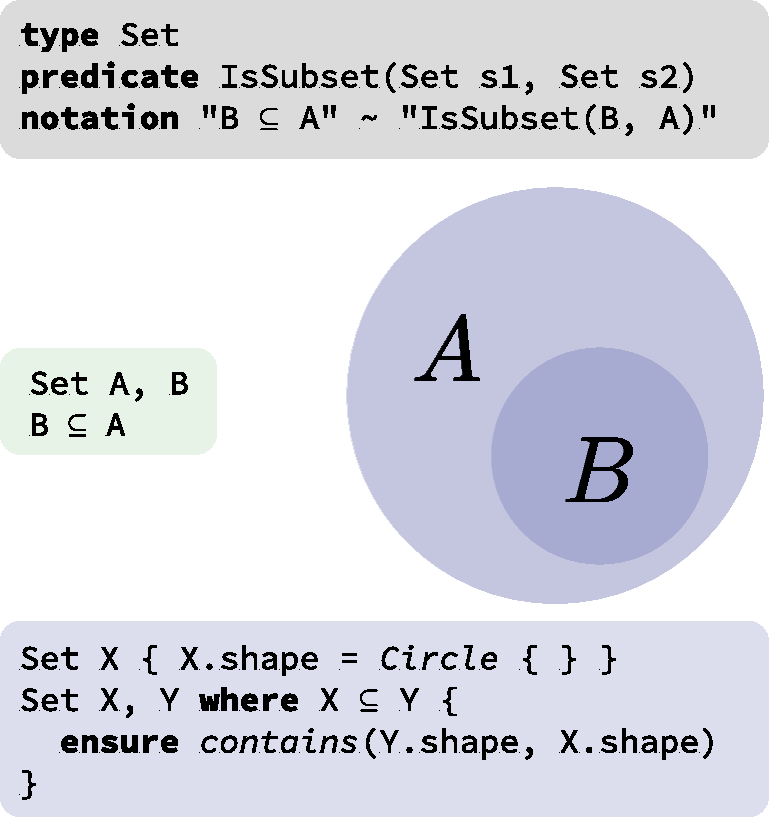
\includegraphics[width=0.45\textwidth]{assets/chapter-2/penrose-trio.pdf}
%   \end{center}
% \end{wrapfigure}

% Instead of a limited focus on one specific domain (as in GraphViz~\cite{graphviz} for graph theory or GroupExplorer~\footnote{\url{https://github.com/nathancarter/group-explorer}} for group theory), \Penrose is extensible to user-defined domains of diagramming. Both \Substance and \Style are parametrized by a \colorbox[HTML]{DBDBDB}{\Domain} schema that defines all possible objects (\eg, \sub{Set}) and relations (\eg, \sub{IsSubset}) in a particular domain, which can be used by associated \Substance and \Style programs. In addition to user-extensibility, a formally encoded domain also enables automatic generation of \Penrose diagrams. 

% \Penrose compiles a \textbf{trio} of \Domain, \Substance, and \Style into a constrained optimization problem defined by a set of graphical constraints (\eg, arrows that represent vectors should start from the origin). The optimization problem is in standard form, \ie, minimization of an objective function subject to equality and inequality constraints~\cite{convexOptimization}. Such problems may be solved with many standard methods. \Penrose currently uses an exterior point method~\cite{exteriorPoint} that starts with an infeasible point and pushes it toward a feasible configuration via progressively stiffer penalty functions---mirroring a process often used by hand.

% The design of \Penrose is driven by the design goals of reuse and scalability, and therefore is suitable for large-scale generation of visual content. The system is scalable and reusable in several dimensions:
    
% % \setlength{\columnsep}{1em}
% % \setlength{\intextsep}{0em}
% % \begin{wrapfigure}{r}{.45\textwidth}
% % \vspace{-10pt}
% %   \begin{center}
% %     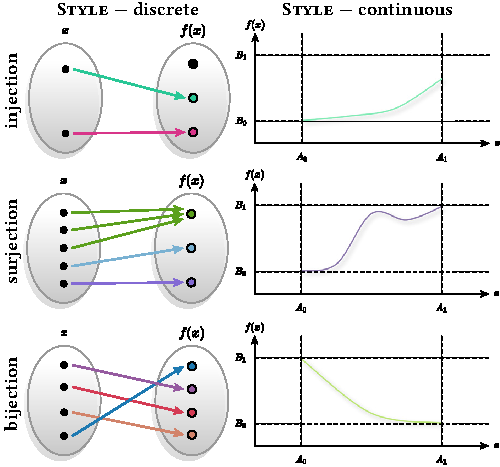
\includegraphics[width=0.45\textwidth]{assets/chapter-2/func-continuous-discrete-vert.pdf}
% %   \end{center}
% % \end{wrapfigure}

% \vspace{1em}
% \begin{figure}[h]
% \begin{minipage}[b]{0.48\linewidth}
% $\bullet$ The optimization problem produced by \Penrose often has multiple solutions, and each point in the solution space corresponds to an alternative diagram. No program changes are required to generate these alternatives.
%     \vspace{3pt}

% $\bullet$ For a visual representation encoded by a \Style program, a wide range of notations (\ie, \Substance programs) can be visualized without any changes to \Style. In the figure on the left, a single discrete \Style program is used to visualize three \Substance programs that describe injective, surjective, and bijective functions.
%     \vspace{3pt}

% $\bullet$ Conversely, multiple \Style{} programs can be applied to the same \Substance{} program, generating alternative visual representations of the same underlying entities. The \Substance programs in the figure are also visualized by an alternative continuous \Style.
% \end{minipage}
% \hfill
% \begin{minipage}[b]{0.5\linewidth}
%     \centering
%     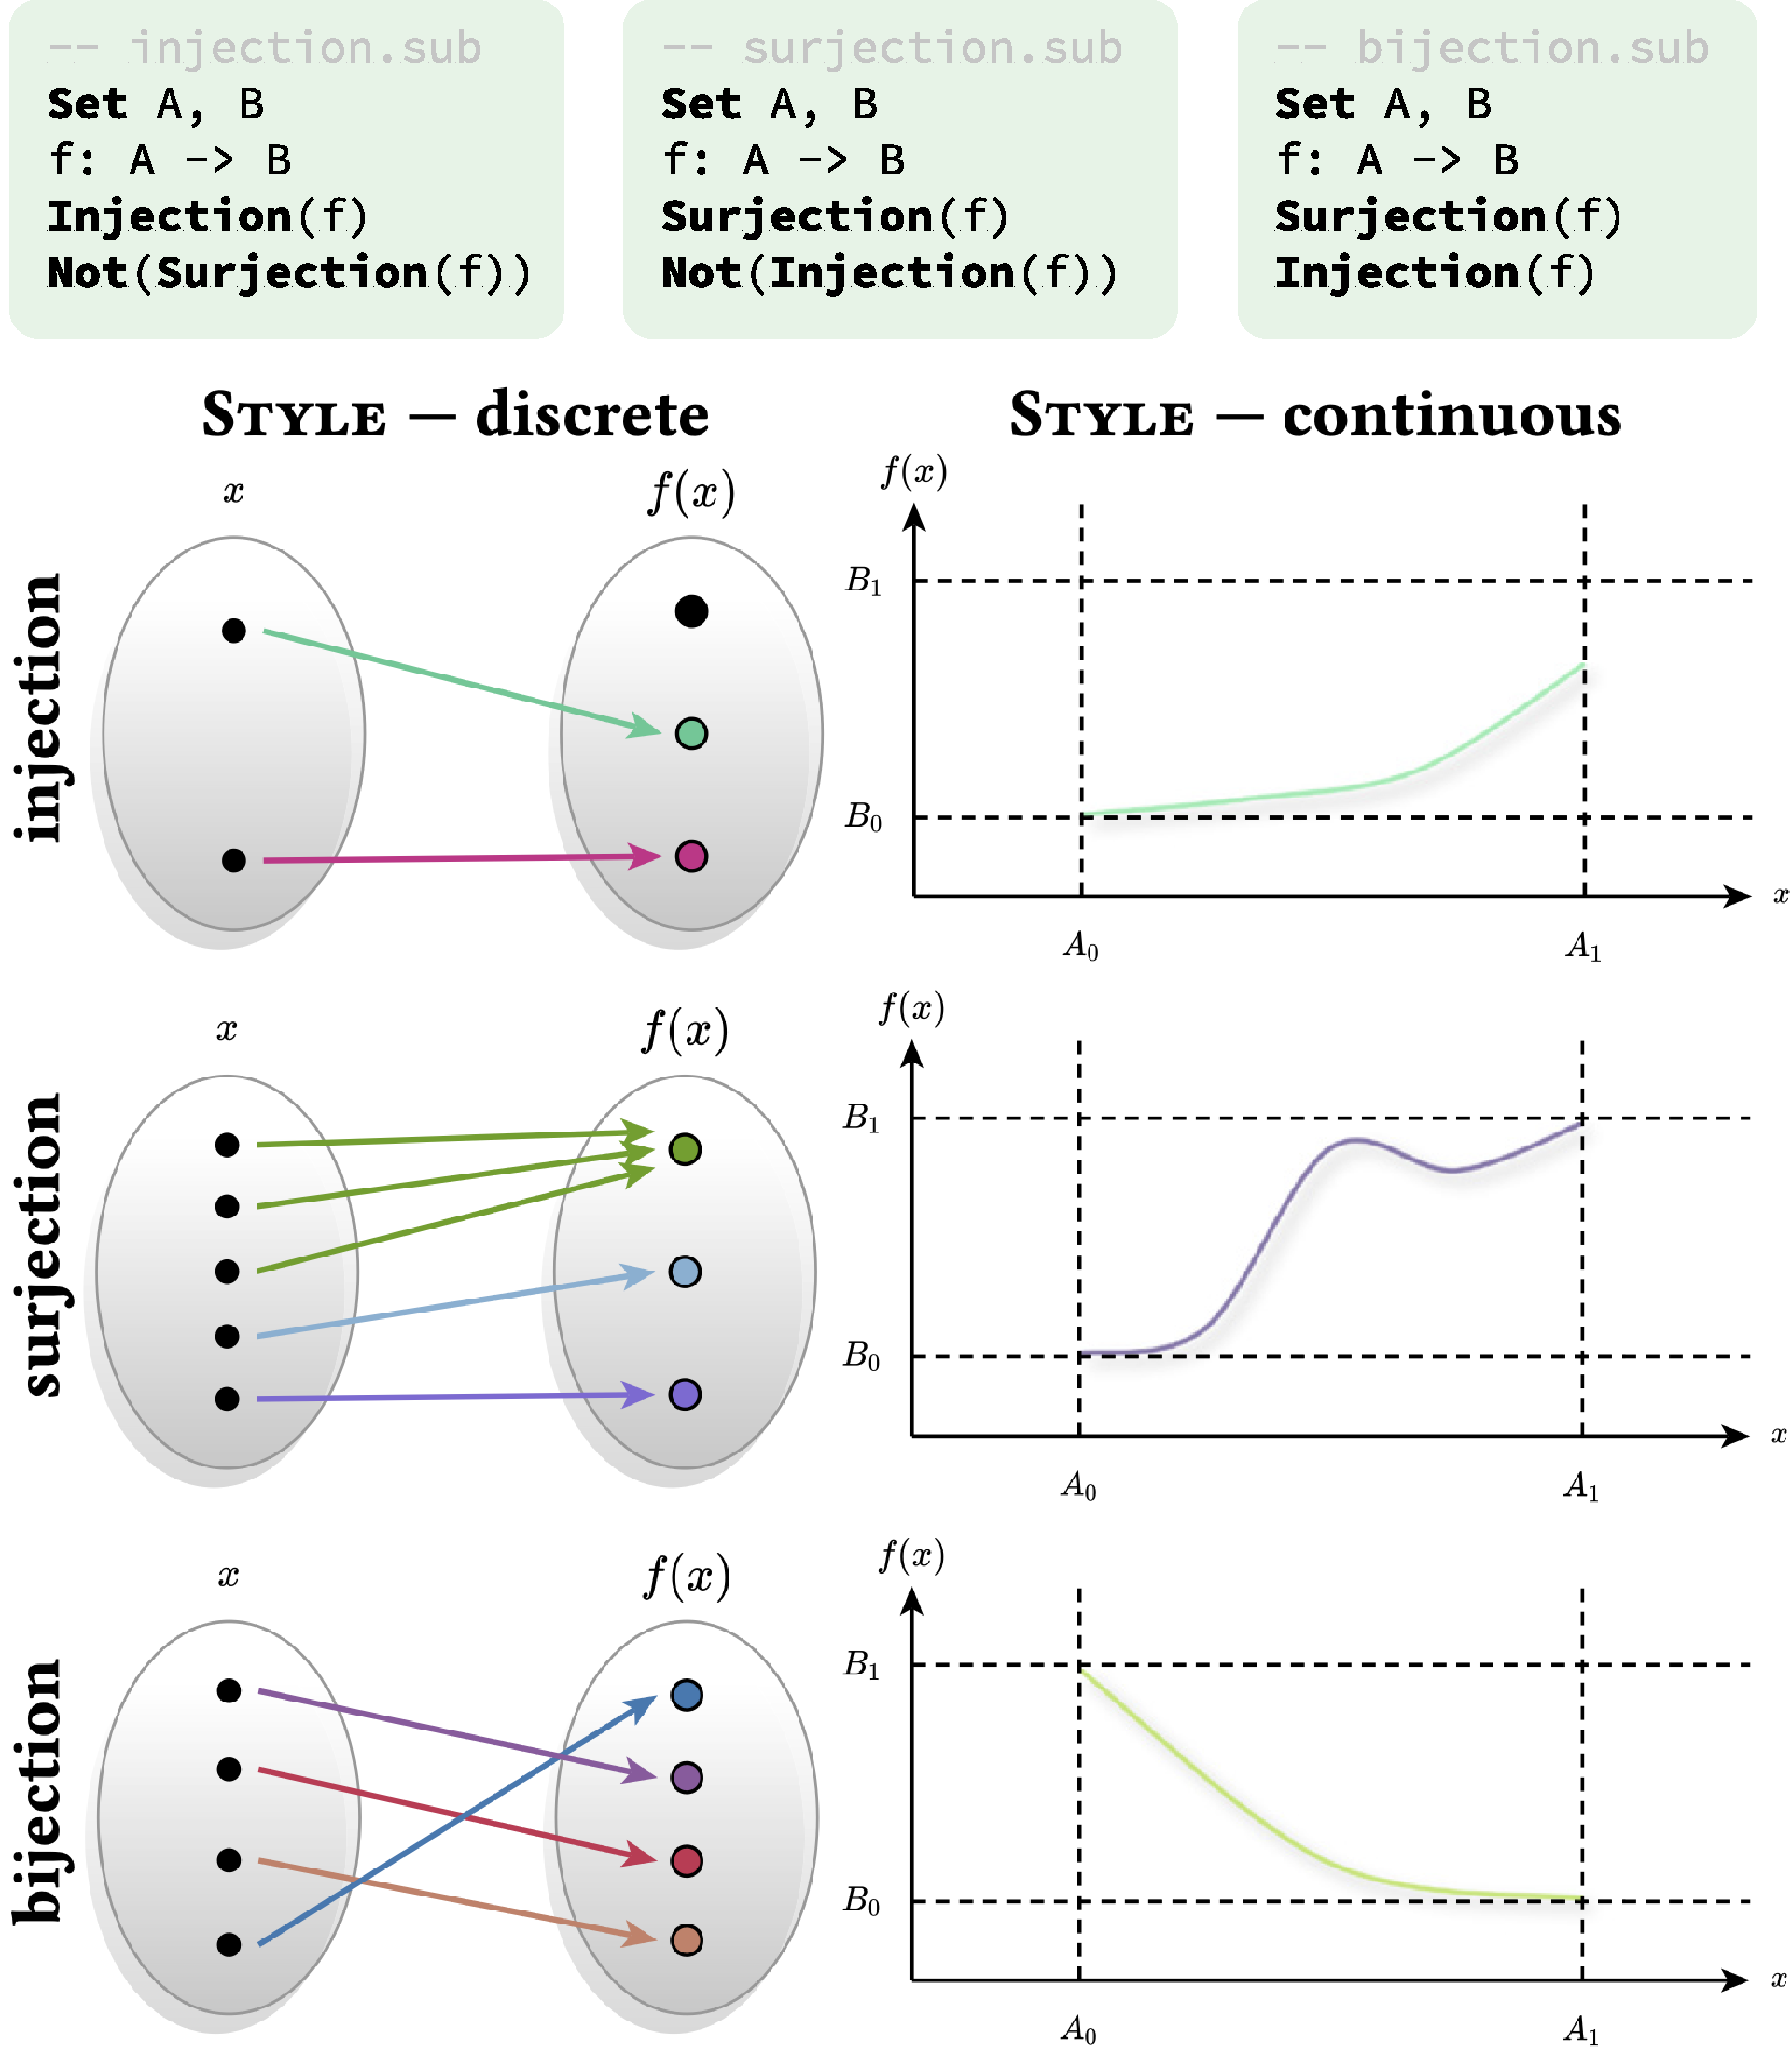
\includegraphics[width=\textwidth]{assets/chapter-2/injection-surjection-bijection.pdf}
% \end{minipage}
% \end{figure}
    
% With the extensible design, \Penrose can automatically generate diagrams from many different domains using familiar syntax. \Penrose-generated geometry, real analysis, ray-tracing, set theory, and algebra are shown below.

% \vspace{10pt}
% 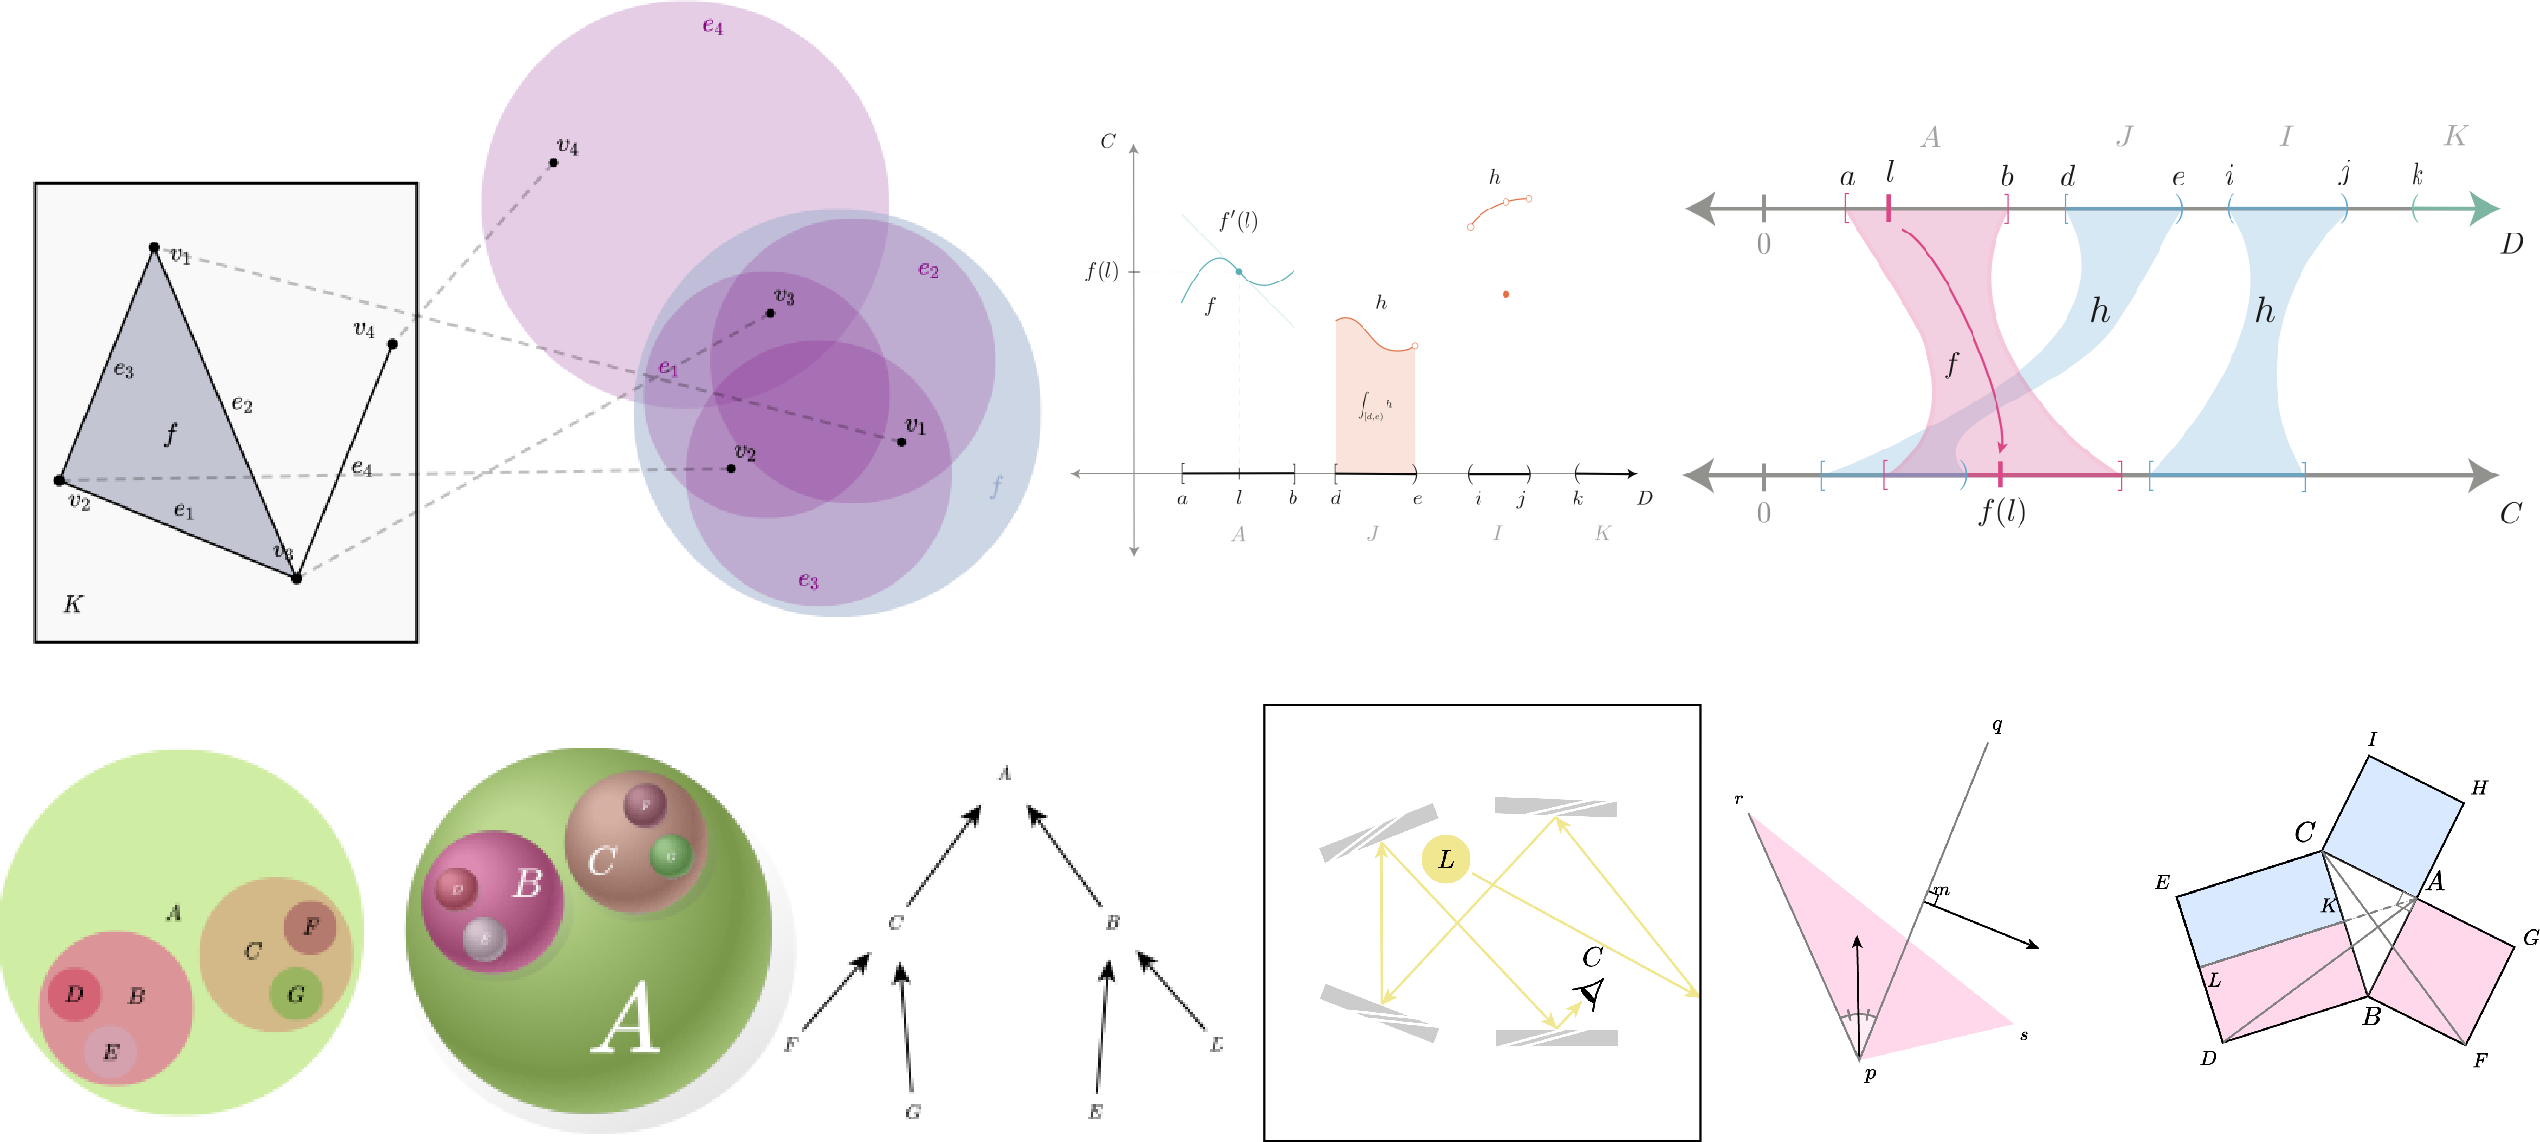
\includegraphics[width=0.95\linewidth]{assets/chapter-2/gallery.pdf}